%!TEX root = ../tudkom_students__201804_v1.4.tex
\chapter{Design und Planung}
\label{ch:design}
%This chapter should describe the design of the own approach on a conceptional level without mentioning the implementation details.
% 5 pages
Um das Vorhaben umzusetzen, müssen zuerst die Anforderungen bestimmt, einige Entscheidungen getroffen und erste Pläne entworfen werden.

\section{Anforderungen}
Als Komponenten werden hauptsächlich eine IMU und eine kompatible MCU, die Daten über BLE übertragen kann sowie für zukünftige Tests auch BT Mesh unterstützt, benötigt.
Die Komponenten sollen ähnliche Anforderungen an die Spannungsversorgung besitzen wie eine Lithiumknopfzelle sie bereitstellen kann, damit kein zusätzlicher Spannungsregler benötigt wird.
Ferner sollen die in der Abschnitt \ref{ch:aims} festgelegten Ziele angestrebt werden.

\section{Energieversorgung}
Zu den typischen mobil verfügbaren Spannungsquellen gehören wiederaufladbare Akkus und Einwegbatterien, die elektrische Energie chemisch speichern können.
Die Gängigsten basieren auf Nickel oder Lithium, wobei die Lithiumbasierenden wegen der höheren Energiemenge bei gleichem Gewicht und Größe unter dem Gesichtspunkt der Mobilität präferiert werden.
Lithiumakkus benötigen eine Ladeelektronik sowie einen Entladeschutz.
Diese Komponenten nehmen Platz auf der Platine ein, verbrauchen Energie, wodurch die Effizienz sinkt, und verlieren ihre maximale Kapazität mit zunehmenden Alter.
Durch ihre maximale Spannung von 4.2 Volt könnten sie nicht ohne Spannungswandler mit den meisten Komponenten betrieben werden, der wiederum Effizienz einbüßen würde. \cite{site_liion}\\
Deshalb wurden Lithiumknopfzellenbatterien als Energieversorgung gewählt.
Durch ihre flache Bauform können sie platzsparend an Platinen befestigt werden.
Während auf dem Prototyping-Board Platz für eine CR2032-Knopfzelle bereit steht, soll auf dem Evaluationsboard aus praktischen Gründen eine CR2450-Knopfzelle genutzt werden.

\section{Datenübertragung zwischen Wearable und Endgerät}
\label{ch:bleAndMesh}
Um das am Besten geeignete Protokoll zu finden, um die Sensordaten der IMU auf die Endgeräte zu übertragen, wurden verschiedene Protokolle verglichen und nach dem Ausschlussverfahren gewählt.\\
Eine drahtgebundene Datenübertragung ist schnell und sehr energiesparend und es sind viele verbreitete Anschlüsse spezifiziert.
Die Mobilität ist dabei aber sehr stark eingeschränkt, da Kabel insbesondere beim Sport sehr stören.\\
Während einige drahtlose Kommunikationsprotokolle wie NFC wegen der geringen Reichweite nicht geeignet sind, sind Mobilfunkprotokolle wie LTE wegen zu hoher Reichweite ineffizient \cite{comparison_wifi_lte}.
Die bekannten Protokolle Wi-Fi und Bluetooth arbeiten unter anderem auf der 2.4-GHz Antenne, weswegen Peer-to-Peer(P2P) Protokolle auf dieser Frequenz in Tabelle \ref{tab:p2p_protocols} vergleichen wurden.\\
\begin{minipage}{\linewidth}
        \renewcommand\footnoterule{}
        \renewcommand{\thefootnote}{\alph{footnote}}
	\captionof{table}{P2P-Protokolle auf der 2.4-GHz Frequenz}
	\label{tab:p2p_protocols}
	\begin{tabularx}{\linewidth}{>{\hsize=.3\hsize}X|>{\hsize=.5\hsize}X|X}
		Protokoll & Typische Anwendung & Kommentar\\
		\hline
		Wi-Fi Hotspot & Teilen der Internetverbindung in einem lokalem Netzwerk & Am Smartphone kann ein Hotspot erstellt werden, die Wearables könnten ihn suchen und sich verbinden, woraufhin z.B. über eine REST-API kommuniziert werden kann.
		Es kann auch die 5-GHz Frequenz genutzt werden.\\
		Wi-Fi Direct & P2P-Kommunikation & Wie Wi-Fi Hotspot aber die Wearables bekommen keinen Internetzugriff vom Smartphone.\\
		Bluetooth (BT) & Datenübertragung, Audiostreaming & Nicht für niedrigen Energieverbrauch ausgelegt.\\
		BT Low Energy (BLE) & P2P-Kommunikation mit geringem Energieverbrauch, z.B. Smartwatches & Während die maximale Geräteanzahl nicht vom Protokoll spezifiziert ist, ist sie in Android auf 7 Geräte beschränkt\footnotemark[1].
		Weiterhin ist die Anzahl zum Beispiel durch die Auslastung der Geräte und des Funkkanals begrenzt.\\
		BT Mesh & Mesh-Kommunikation mit geringem Energieverbrauch & Nachrichten werden hierbei über das gesamte Netzwerk geflutet, wodurch die Reichweite des Netzwerkes erhöht wird und die Auslastung auf das Netzwerk verteilt wird aber der Energieverbrauch aller Knoten steigt.
		BLE Geräte können mit Mesh-Netzwerken kompatibel gemacht werden, indem sie sich zu einem Knoten des Netzwerks verbinden.\\
		Thread, ZigBee & Smarthome & Nicht ohne weitere Hardware unter Android\\
		Ant, Ant+ & Sen\-sor\-da\-ten\-über\-tra\-gung mit geringem Energieverbrauch & Nicht von allen Smartphones ohne zusätzliche Hardware unterstützt\\
	\end{tabularx}
	\footnotetext[1]{Beschränkung durch GATT\_MAX\_PHY\_CHANNEL \cite{site_androidBlTarget}}
\end{minipage}\\\\
Da Bluetooth nicht für einen geringen Energieverbrauch ausgelegt ist, werden die Alternativen BLE und BT Mesh bevorzugt.
Die Smarthome Protokolle funktionieren ohne zusätzlicher Hardware nicht am Smartphone.
Ant und Ant+ sind zwar für die Sensordatenübertragung bei Smartphones ausgelegt, aber brauchen zusätzlich ein Dongle, wenn sie das Protokoll nicht unterstützen.
Sowohl handelsübliche Laptops als auch das vorliegende Smartphone, ein Pocophone F1, unterstützt die Protokolle nicht.\\
"BLE ist etwa 30\% energieeffizienter als Wi-Fi"\footnote{Übersetzung durch den Verfasser} \cite{comparison_wifi_ble}, weswegen die Wi-Fi Protokolle heraus fallen.
BT Mesh löst zwar das Problem der Geräteanzahlbeschränkung unter Android, allerdings auf Kosten des Energieverbrauchs.
Die erweiterte Reichweite durch das Mesh-Netzwerk wird bei einem Wearable in der Regel nicht benötigt.\\
Die Datenübertragung zwischen Wearable und Endgerät soll mit BLE stattfinden, da dieses Protokoll von fast jedem Smartphone und Laptop unterstützt wird und den Anforderungen erfüllen kann.
Zusätzlich soll BT Mesh als Option offen gelassen werden, da es gegebenenfalls auftretende Probleme mit BLE lösen kann.
Der zusätzliche Energieverbrauch durch das Mesh-Netzwerk müsste zunächst evaluiert werden.

\section{Wahl der Hauptkomponenten}
Die Arbeit hat sich zunächst danach gerichtet Komponenten zu wählen, die es auf fertige Platinen gelötet gibt, da sich QFN-Komponenten händisch nicht löten lassen.\\
Da sich der Energieverbrauch von MCUs anhand der Datenblätter schlecht vergleichen lässt, wurde betrachtet, welche Komponenten sich oft zusätzlich auf den Platinen befinden aber viel Strom verbrauchen.
In einem Blog \cite{site_arduinolp} wurden verschiedene Komponenten von einem Arduino Pro Mini entfernt und deren Auswirkungen auf den Stromverbrauch ermittelt.
Das Entfernen der LED, die dauerhaft leuchtet um den Betrieb anzuzeigen, hat eine Einsparung von mehr als 15 \% bei aktiver Nutzung bewirkt und mehr als 90 \% im Schlafmodus der Recheneinheit.
Das Entfernen des Spannungsreglers hat mindestens weitere 9 \% bei Nutzung und 75 \% im Standby eingespart.
Ein anderer Blog \cite{site_arduinolp2} beschreibt, dass ein integrierter Programmierer zwar einen einfach zu verwendenden USB Anschluss bietet, aber gleichzeitig die Stromaufnahme verdreifachen kann.
Während eine LED problemlos zu entfernen ist, wurde auf die anderen beiden Bauteile nach Möglichkeit verzichtet, da ein Entfernen auch die Funktion der Platine einschränken oder die Platine zerstören kann.

\subsection{MCU}
\label{ch:mcu}
Die Bluetooth SIG, die das Bluetooth Protokoll spezifiziert, hat eine Liste mit geprüften Implementierungen von BT Mesh veröffentlicht \cite{site_qualifiedMesh}.
Mit dieser Liste wurden die Herstellerseiten nach passenden verfügbaren MCUs durchsucht bis die Wahl auf die nRF52832 MCU gefallen ist.
Die MCU war schon in den zwei fertigen Produkten von Arduino und aconno enthalten weswegen von einer hohen Bekanntheit auszugehen ist.\\
Der nRF52832 hat eine Spannungsanforderung von 1.7 bis 3.6 V, wodurch er sich direkt an einer Knopfzelle betreiben lässt.
Das EasyDMA-Modul enthält einen Buffer um SPI- und I2C-Kommunikation abzuhandeln, während die MCU im Schlafmodus ist.
Das schwächere Modell nRF52810 unterstützt BT Mesh nicht.
Das stärkere Modell nRF52840 hat mehr Speicherplatz und unterstützt weitere Protokolle aber verbraucht dementsprechend mehr Energie. \cite{site_nrfProducts}\\
Durch den Pinabstand von 2.54 mm, wie er sich auch auf Arduinos vorfindet, ist die Platine von SparkFun sehr einfach zu verwenden.
Sie enthält eine Power-LED, die sich über JP6 trennen lässt.
Es existiert ein Spannungsregler, der sich überbrücken lassen müsste.
Die Platine stellt eine Alternative dar, falls sich mit den kleineren Platinen wegen der Größe nicht mehr arbeiten lassen würde.
Die Größe dieser Platine ist nicht direkt angegeben, aber wegen des Pinabstands mindestens 15 x 43 mm. \cite{datasheet_nrfSpark}\\
Der ACN52832 von aconno enthält weder Power-LED noch Spannungsregler sondern nur die nötigsten Komponenten.
Er hat eine Größe von 20 x 24.8 mm. \cite{datasheet_nrfAcn}\\
Der BL651 von Laird enthält ebenfalls nur die nötigsten Komponenten und hat eine Größe von 10 x 14 mm \cite{datasheet_nrfLaird}.
Es existieren noch weitere Platinen vom nRF52832 sodass eine sehr gute Verfügbarkeit gegeben ist.
Sollte eine Platine nicht mehr erhältlich sein, könnte sie durch eine Andere ersetzt werden, da die Platinen nur die Pins vom nRF52832 besser zugänglich machen und die nötigen Taktgeber, Kondensatoren und Antennen bereitstellen sollen.
Für den Prototypen wurde zunächst das nRF52 DK von Nordic verwendet, da es auch den externen Programmierer für die Platinen enthält und die Pins ohne zu Löten mit Jumperkabel verbunden werden können.

\subsection{IMU}
Auf der Suche nach einer passenden IMU haben sich der STMicroelectronics LSM6DSL und Bosch BMI260 als besonders energiesparend hervorgetan.
Der LSM6DSL läuft mit 1.71 - 3.6 V, verbraucht 0.4 mA im normalen Modus und 0.65 mA im Performance-Modus \cite{datasheet_lsm6dsl}. Die zugehörige Platine STEVAL-MKI178V2 enthält keine überflüssigen Komponenten.\\
Der BMI260 läuft mit 1.7 - 3.6 V und verbraucht 0.685 mA
Der Sensor war zu Beginn der Arbeit angekündigt.
Da er pinkompatibel zum Vorgänger BMI160 ist, wurde mit dem BMI160 entwickelt.
Zum Ende der Arbeit sollte er durch den BMI260 getauscht werden, aber leider war er da nicht verfügbar. \cite{site_bmi260}\\
Der BMI160 läuft auch mit 1.7 - 3.6 V aber verbraucht 0.925 mA \cite{datasheet_bmi160}.
Das BMI160 Shuttle Board enthält zusätzlich einen BMM150 Magnetometer.
Der Magnetometer hat im Standby einen Verbrauch von 1 $\mu$A, kann aber mechanisch entfernt werden \cite{datasheet_bmm150}.\\
Beide IMUs haben einen FIFO-Buffer eingebaut.
Die gemessenen Daten können in dem Buffer hinterlegt werden, sodass die MCU die Daten in Bursts lesen und länger im Schlafmodus bleiben kann, da ein Wechsel der Energiemodi wiederum Energie kostet.\\
Mit zwei Interrupt Pins können die IMUs die MCU über bestimmte Events informieren.
Das DataReady-Event benachrichtigt, wenn der Sensor neue Daten gemessen hat.
Das FIFO-Watermark- oder FIFO-Threshold-Event wird geworfen, wenn die FIFO über einen eingestellten Prozentsatz gefüllt ist.
Das FIFO-Full-Event zeigt an, dass die FIFO komplett gefüllt ist.
Für spezielle Anwendungen unterstützen beide IMUs weitere Events, wie das Significant-Motion-Event um ein Aufheben des Sensors durch einen Nutzer zu melden.\\
Da die Platinen der IMUs wegen ihrer Größe nicht optimal sind und zukünftige Anwendungen bessere Sensoren oder einen eingebauten Magnetometer benötigen können, soll der Code modular aufgebaut sein, sodass das Sensormodell einfach getauscht werden kann.

\section{Zusammenwirken der Komponenten}
Während SPI 4 Datenverbindungen braucht, braucht I2C 2 Datenverbindungen.
Da die Pins in der Software der MCU zugewiesen werden, kann für SPI verkabelt und die selbe Verdrahtung auch für I2C genutzt werden.
Abbildung \ref{fig:abstract_schema} stellt die Verbindungen graphisch dar.\\
Wenn das Wearable nicht mit einem Endgerät verbunden ist, soll es in den Schlafmodus wechseln.
Über einen Knopf soll es aufgeweckt werden und mit dem Advertisen beginnen.
Mit dem Knopf soll das Advertisen auch wieder abgebrochen werden und das Wearable in den Schlafmodus versetzt werden können.
Wenn das Wearable mit einem Endgerät verbunden ist, soll es sich trennen lassen, indem der Knopf über einige Sekunden gedrückt gehalten wurde, damit es sich nicht versehentlich trennt.\\
Um dem Nutzer ein Feedback über den Status zu geben, soll eine LED verwendet werden.
Die LED soll beim Advertisen in regelmäßigen Abständen blinken, sodass sich der Stromverbrauch nicht wie bei einer immer angeschalteten Power-LED auswirkt.
Wenn eine Verbindung hergestellt wurde, soll eine zweite LED zu Beginn der Verbindung aufblinken.
Wenn während einer Verbindung kurz auf den Knopf gedrückt wird, soll die zweite LED kurz aufleuchten.
\begin{figure}[hbtp]
	\centering
	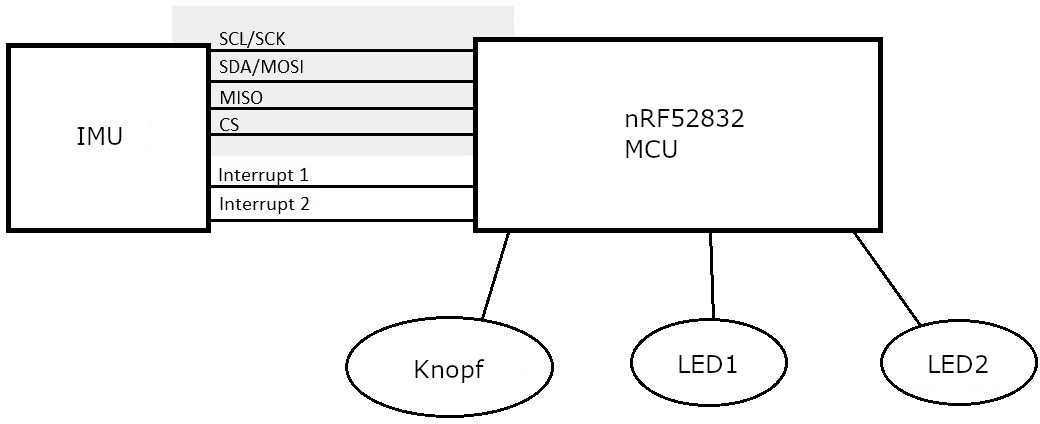
\includegraphics[width=0.9\linewidth]{res/schemaAbstrakt.jpg}
	\caption{Veranschaulichung der Verbindungen der benötigten Komponenten}
	\label{fig:abstract_schema}
\end{figure}

\section{BLE Schnittstelle}
In einer Characteristic sollen die 3 Achsen des Beschleunigungssensors, die 3 Achsen des Gyrosensors und der Zeitstempel hinterlegt werden.
Damit soll sich der Bewegungsablauf des Sensors zeitlich korrekt rekonstruieren lassen, da BLE die Daten in Burst mit Zeitabständen vom Connection-Interval übergibt und die Daten in Burst von der FIFO abgerufen werden können.
Um die MCU möglichst selten aus dem Schlafmodus zu holen, soll die FIFO der IMU in den Buffer der EasyDMA geleert werden, sobald sie komplett gefüllt ist.
Zusätzlich soll umgefüllt werden, wenn die MCU durch andere Interrupts die z.B. durch den BLE-Stack aufgeweckt wird.
Der Wert der Characteristic soll von der MCU nur gelesen werden können, aber es soll das Notify-Bit gesetzt werden können.\\
Mit einer zweiten Characteristic soll sich die Abfragerate der IMU einstellen lassen.
Da die Sensorabfragerate damit von der Datenübertragungsrate unabhängig ist, lässt sich die Energieaufnahme getrennt evaluieren.
Während eine niedrige Sensorabfragerate mit einer hohen Datenübertragungsrate sehr geringe Latenzen der Sensordaten ermöglicht, sind hohe Sensorabfrageraten mit niedrigen Datenübertragungsraten bei weniger zeitkritischen Anwendungen zur intensiven Auswertung interessant.
Damit die Verbindung aufrecht erhalten werden aber die Datenerfassung pausiert werden kann, soll die IMU über die Characteristic auch kurzzeitig ausgeschaltet werden können.
Die zweite Characteristic soll von der MCU gelesen und geschrieben werden können, sowie das Endgerät bei Änderungen benachrichtigt werden.

\section{Applikation des Android Smartphones}
Beim Start der App soll nach den Wearables gesucht und zu den Wearables verbunden werden.
Bei einer Verbindung soll das Notify-Bit der Characteristics gesetzt werden, damit neue Daten beim Smartphone ankommen.
Um einschätzen zu können, ob die empfangenen Daten korrekt erfasst werden und ankommen, sollen die Sensordaten und Statistiken zur Verbindung graphisch dargestellt werden.
Da es im Android SDK keine einfache Möglichkeit dazu gibt, soll die Bibliothek Androidplot\footnote{\url{http://androidplot.com/}, abgerufen am 10.07.2019} genutzt werden.
Der Wert der zweiten Characteristic soll gesetzt und die Verbindungsdatenrate geändert werden können.
